\documentclass[conference]{IEEEtran}
\IEEEoverridecommandlockouts
%The preceding line is only needed to identify funding in the first footnote. If that is unneeded, please comment it out.
\usepackage{amsmath}
\usepackage{amsfonts}
\usepackage{amssymb}
%\usepackage{mdframed}
\usepackage{framed}
\usepackage{algorithmic}
\usepackage{algorithm}
\usepackage{setspace}
\usepackage{graphicx}
\usepackage{textcomp}
\usepackage{hyperref}
\hypersetup{
    colorlinks,
    citecolor=blue,
    linkcolor=red,    
    urlcolor=red,
}
\usepackage{multicol}
\usepackage{multirow, bigdelim}
\usepackage{tcolorbox}
\usepackage{xcolor}
\usepackage{longtable}
\usepackage[backend=biber,style=ieee]{biblatex} % or \usepackage[numbers]{natbib}
\addbibresource{references.bib} % for biblatex
\newcommand{\norm}[1]{\left\lVert#1\right\rVert}
\usepackage{nomencl}
\usepackage{ifthen}
  \renewcommand{\nomgroup}[1]{%
  \item[\bfseries
  \ifthenelse{\equal{#1}{B}}{Notations}{%
  \ifthenelse{\equal{#1}{A}}{Abbreviations}{}}%
  ]}
\renewcommand{\nomname}{\bfseries Nomenclature}
\usepackage{cleveref}


\usepackage{tikz}
\usetikzlibrary{shapes.geometric, arrows}
\tikzstyle{process} = [rectangle, rounded corners, minimum width=4cm, minimum height=1cm, text centered, draw=black]
\tikzstyle{decision} = [diamond, minimum width=4cm, minimum height=1cm, text centered, draw=black]
\tikzstyle{arrow} = [thick,->,>=stealth]




\begin{document}
\title{Optimal Allocation with Multi Wholesale Market Value Stacking of Distributed Energy Resources \\
(2025 UpSCAleDEV TotalEnergies) \\}
\author{\IEEEauthorblockN{Yizhan Gu} \\
\IEEEauthorblockA{\textit{Center for Energy Research} \\ \\
\textit{University of California, San Diego}\\
\textit{9500 Gilman Dr, La Jolla, CA 92093, USA}\\
\textit{Email: {yig031}@ucsd.edu}
}}


\maketitle
\thispagestyle{plain}
\pagestyle{plain}
\makenomenclature
\setlength{\nomitemsep}{-\parskip}
\renewcommand*\nompreamble{\begin{multicols}{2}}
\setlength{\parindent}{1em}
\renewcommand*\nompostamble{\end{multicols}}


\begin{table*}[ht]   
\begin{framed}
\footnotesize
 
\nomenclature[A]{EV}{Electric Vehicle}
\nomenclature[A]{MPC}{Model Predictive Control}
\nomenclature[A]{BESS}{Battery Energy Storage System}
\nomenclature[A]{LMP}{Locational Marginal Price}
\nomenclature[A]{PV}{Photovoltaic}
\nomenclature[A]{CAISO}{California Independent System Operator}
\nomenclature[A]{UCSD}{University of California San Diego}
\nomenclature[A]{DR}{Demand Response}
\nomenclature[A]{DER}{Distributed Energy Resource}
\nomenclature[A]{DRAM}{Demand Response Auction Mechanism}
\nomenclature[A]{ELRP}{Emergency Load Reduction Program}
\nomenclature[A]{AT}{Arrival Time of EV}
\nomenclature[A]{DT}{Departure Time of EV}
\nomenclature[A]{ED}{Energy Demand of EV}
\nomenclature[A]{AS}{Ancillary Service}
\nomenclature[A]{AGC}{Automatic Generation Control}
\nomenclature[A]{SDG\&E}{San Diego Gas \& Electric}
\nomenclature[A]{DA}{Day-ahead}
\nomenclature[A]{RT}{Real-time}
\nomenclature[A]{SOC}{State of charge}
\nomenclature[A]{SLR}{Service level reduction}




%%%%%%%%%%%%%%%%%%%%%%%%%%%%%%%%


\nomenclature[B]{$Cost_t$}{total cost of the aggregator at $t$ [$\$$]}
\nomenclature[B]{$Revenue_t$}{total revenue of the aggregator at $t$ [$\$$]}
%\nomenclature[B]{$x_t$}{sample variable [dimensionless]}
\nomenclature[B]{$N_{\text{EV}}$}{number of EVs [dimensionless]}
\nomenclature[B]{$N$}{number of all time steps in MPC [96, dimensionless]}
\nomenclature[B]{$T$}{MPC running time horizon [24, hour]}
\nomenclature[B]{$t$}{current time step %in real life 
[dimensionless]}
\nomenclature[B]{$k$}{index for time step in MPC loop [dimensionless]}
\nomenclature[B]{$i$}{index for EV [dimensionless]}
\nomenclature[B]{$d_i$}{days belonging to the  baseline calculation [dimensionless]}
\nomenclature[B]{$\Delta{t}$}{length of time step [0.25, hour]}
\nomenclature[B]{$X_{t,\text{opt}}$}{matrix of optimal EV charging power for the rest of the day at $t$ [$(T-t+1) \times N_{\text{EV}}$, kW]}
\nomenclature[B]{$L_{\text{imp},t}^{\text{EV}}$}{implemented EV load at $t$ [kW]}
\nomenclature[B]{$L_{\text{imp},t}^{\text{EV}}$}{implemented EV load with $\eta$ service level at $t$ [kW]}
\nomenclature[B]{$L_{\text{bid},h}^{\text{EV}}$}{EV load bid at $h$ [kW]}
\nomenclature[B]{$\pmb{\eta}_{N_{\text{EV}}}$}{charging service level vector of EV [$N_{\text{EV}} \times 1$, dimensionless]}
\nomenclature[B]{$N_{\text{days}}$}{number of days used in  baseline calculation [dimensionless]}
\nomenclature[B]{$L^{\text{B}}_t$}{demand response baseline load at $t$ [kW]}
\nomenclature[B]{$L^{\text{historical}, d_i}_t$}{grid load of UCSD aggregator on day $d_i$ at $t$ [kW]}
\nomenclature[B]{$L^{\text{building}}_t$}{buildings load at $t$ [kW]}
\nomenclature[B]{$P^{\text{PV}}_t$}{solar PV generation at $t$ [kW]}
\nomenclature[B]{$P^{\text{D}}_t$}{battery discharging power at $t$ [kW]}
\nomenclature[B]{$L^{\text{net}}_{\text{act},t}$}{actual net load of aggregator at $t$ [kW]}
\nomenclature[B]{$L^{\text{net}}_{\text{bid},h}$}{net load of aggregator bid to CAISO at $h$ [kW]}
\nomenclature[B]{$L_{\text{forecast},h}^{\text{building}}$}{forecast building load at $h$ [kW]}
\nomenclature[B]{$P^{\text{PV}}_{\text{forecast},h}$}{forecast solar PV generation at $h$ [kW]}
\nomenclature[B]{$P^{\text{BESS}}_{\text{bid}, h}$}{battery load bid to CAISO at $h$ [kW]}
\nomenclature[B]{$P^{\text{BESS}}_t$}{real-rime battery load at $t$ [kW]}
\nomenclature[B]{$P_{\text{act},t}^{\text{DR}}$}{actual demand response capacity at $t$ [kW]}
\nomenclature[B]{$P_{\text{bid},h}^{\text{DR}}$}{demand response capacity bid to CAISO at $h$ [kW]}
\nomenclature[B]{$c_{\text{NCD}}$}{real-time non-coincident demand rate [$\$$/kW]}
\nomenclature[B]{$c_{\text{PD}}$}{real-time peak demand rate [$\$$/kW]}
\nomenclature[B]{$c_{\text{TOU}}$}{real-time time-of-use energy rate [$\$$/kWh]}
\nomenclature[B]{$\bar{L}^{\text{net}}_{\text{NCD}}$}{highest non-coincident demand in the current month [kW]}
\nomenclature[B]{$\bar{L}^{\text{net}}_{\text{PD}}$}{highest peak demand in the current month [kW]}
\nomenclature[B]{$z_t^{\text{PD}}$}{peak demand binary indicator at $t$ [1 or 0, dimensionless]}
\nomenclature[B]{$\delta$}{penalty coefficient for EV energy demand deviation at $t$ [1000, dimensionless]}
\nomenclature[B]{$z_{\text{event},h}^{\text{DR}}$}{demand response event binary indicator at $h$ [1 or 0, dimensionless]}
\nomenclature[B]{$c_{\text{EV}}$}{EV charging rate paid by drivers [$\$$/kWh]}
\nomenclature[B]{$c_{\text{LMP},t}^{\text{DA}}$}{day-ahead LMP at $t$ [$\$$/kWh]}
\nomenclature[B]{$c_{\text{LMP},t}$}{real-time LMP at $t$ [$\$$/kWh]}
\nomenclature[B]{$R^{\text{AS}}_t$}{battery ancillary service energy payment at $t$ [$\$$/h]}
\nomenclature[B]{$S_t^{\text{DR}}$}{revenue from demand response settlement at $t$ [$\$$/h]}
\nomenclature[B]{$P^{\text{C}}_t$}{battery charging power at $t$ [kW]}
\nomenclature[B]{$P^{\text{RU}}_t$}{battery regulation up power to the grid at $t$ [kW]}
\nomenclature[B]{$P^{\text{RD}}_t$}{battery regulation down power from the grid at $t$ [kW]}
\nomenclature[B]{$P^{\text{SP}}_t$}{battery spinning reserve power to the grid at $t$ [kW]}
\nomenclature[B]{$P^{\text{NSP}}_t$}{battery non-spinning reserve power to the grid at $t$ [kW]}
\nomenclature[B]{$c_{\text{RU}}$}{real-time regulation up rate [$\$$/kWh]}
\nomenclature[B]{$c_{\text{RD}}$}{real-time regulation down rate [$\$$/kWh]}
\nomenclature[B]{$c_{\text{SP}}$}{real-time regulation up rate [$\$$/kWh]}
\nomenclature[B]{$\gamma_{\text{RU}}$}{regulation up efficiency [0.25, dimensionless]}
\nomenclature[B]{$\gamma_{\text{RD}}$}{regulation down efficiency [0.25, dimensionless]}
\nomenclature[B]{$\alpha^{\text{SP}}_t$}{spinning reserve binary indicator at $t$ [1 or 0, dimensionless]}
\nomenclature[B]{$\alpha^{\text{NSP}}_t$}{non-spinning reserve binary indicator at $t$ [1 or 0, dimensionless]}
\nomenclature[B]{$P_{\text{max}}^{\text{BESS}}$}{maximum charging or discharging power of battery [250, kW]}
\nomenclature[B]{$SOC^{\text{BESS}}_{\text{min}}$}{minimum state of charge of battery [0\%, dimensionless]}
\nomenclature[B]{$SOC^{\text{BESS}}_{\text{max}}$}{maximum state of charge of battery [100\%, dimensionless]}
\nomenclature[B]{$SOC^{\text{BESS}}_t$}{real-time state of charge of battery [dimensionless]}
\nomenclature[B]{$C^{\text{BESS}}$}{battery capacity [332, kWh]}
\nomenclature[B]{$\gamma_s$}{storage efficiency of battery [1, dimensionless]}
\nomenclature[B]{$\gamma_c$}{conversion efficiency of battery [0.85, dimensionless]}
\nomenclature[B]{$X_{\text{imp}}$}{matrix of implemented EV charging power [$T \times N_{\text{EV}}$, kW]}
\nomenclature[B]{$\hat{e}_t$}{matrix of maximum energy that can be charged to EV at $t$ [$(T-t+1) \times N_{\text{EV}}$, kWh]}
\nomenclature[B]{$\mathbf{1}_{N_{\text{EV}}}$}{vector one [$N_{\text{EV}} \times 1$, dimensionless]}
\nomenclature[B]{$\mathbf{1}_t$}{vector one [$(T-t+1) \times 1$, dimensionless]}
\nomenclature[B]{$c_{\text{bid},h}^{\text{AS}}$}{bidding rate to AS market at $h$ [$\$$/kWh]}
\nomenclature[B]{$c_{\text{bid},h}^{\text{DR}}$}{bidding rate to DRAM market at $h$ [$\$$/kWh]}
\nomenclature[B]{$\bar{c}$}{bid cap of DRAM market [$1, \$$/kWh]}
\nomenclature[B]{$\underline{c_{\text{LMP}}}$}{floor of real-time LMP [$\$$/kWh]}
\nomenclature[B]{$z_{\text{price},h}$}{favorable price binary indicator in EV service level reduction at $h$ [1 or 0, dimensionless]}
\nomenclature[B]{$z_{\text{layover},i,h}$}{layover binary indicator in EV service level reduction [1 or 0, dimensionless]}
\nomenclature[B]{$\eta_i$}{actual charging service level of EV $i$ [dimensionless]}
\nomenclature[B]{$\eta_{\text{min},i}$}{minimum charging service level of EV $i$ [dimensionless]}
\nomenclature[B]{$z^{\text{D}}_t$}{battery discharging binary indicator at $t$ [1 or 0, dimensionless]}
\nomenclature[B]{$L^{\text{B, DA}}_t$}{day-ahead demand response grid baseline at $t$ [kW]}
\nomenclature[B]{$P^{\text{cycle}}_t$}{battery total cycle power at $t$ [kW]}
\nomenclature[B]{$P_t^{\text{AS}}$}{real-time additional ancillary service bid capacity at $t$ [kW]}
\nomenclature[B]{$e_{di}$}{forecast energy demand of EV $i$ at departure [kWh]}
\nomenclature[B]{$e_{ai}$}{energy demand of EV $i$ at arrival [kWh]}




\printnomenclature
\end{framed}
\end{table*}

%%%%%%%%%%%%%%%%%%%%%%%%%%%%%%%%
\section{Abstract}
There is a growing need to charge electric vehicles (EVs) efficiently and counteract the intermittency inherent to greater penetration of variable renewable energy generation in the modern electricity grid. Techniques such as `valley-filling' and 'peak-shaving' to shift load demand from less desirable to more desirable times have received great attention, especially from microgrid operators. Smart charging/discharging of dispatchable energy resources like electric vehicles (EVs) and battery energy storage systems (BESS) can play a very important role to achieve such desirable load shifting to ultimately reduce electricity costs. Additionally, microgrid operators can also choose to participate in different energy markets as an additional revenue stream by leveraging the flexibility in BESS. This study proposes an model predictive control (MPC) framework for the coordinated management of a university campus microgrid composed of local building load, PV generation, BESS and EV charging. With the consideration of wholesale demand response and ancillary services markets, the proposed method dynamically schedules EV and BESS dispatch with forecasts of local load demand, PV generation and EV sessions, enabling the system to simultaneously reduce electricity costs while providing load flexibility. Simulation results using UC San Diego campus data demonstrate that the proposed approach achieves significant cost reductions with respect to the current micro-grid arrangement without MPC optimization or market participation, and leads to significantly lower peaks. 


\section{Literature review}
The increasing penetration of EVs, PV generation, and BESS presents both opportunities and challenges for larger grid stability and profitability of microgrid operators. Prior studies have explored various control strategies to model the energy flows in such systems, particularly under a simplified optimal control framework. Chen et al.~\cite{chen2024cost} proposed an economic MPC algorithm to arrange the charging schedule of each EV respectively with day-ahead (DA) forecast. It also models the virtual trading between an aggregator and the California Independent System Operator (CAISO) on DR products in the DRAM (Demand Response Auction Mechanism) market. Barba et al.~\cite{10761105} emphasizes participation of BESS in the value-stacking market, with a comprehensive classification of energy arbitrage, frequency regulation revenue, and operating reserves revenue. 

...



Moreover, forecast-based EV charging has been studied, but integration with local renewable generation and building loads remains underexplored, especially in the context of dynamic DR signals and AS commitments in the wholesale electricity market. This paper addresses these gaps by presenting a unified MPC-based optimization framework that (1) co-optimizes EV charging, PV generation, BESS dispatch, and building load, and (2) enables campus-scale participation in DA/RT wholesale energy markets and DR/AS programs in California.

\section{Problem Formulation}

\subsection{Value-stacking Blocks}

\textbf{Objective Function:}
\begin{align}
    &\min_{\substack{X_{t,\text{opt}}, P^{\text{D}}_{t}, P^{\text{C}}_{t}, P^{\text{RU}}_t, P^{\text{RD}}_t, P^{\text{SP}}_t, P^{{\text{NSP}}}_t}} Cost_t - Revenue_t \label{eq:obj}
\end{align}


\textbf{General Notations:}
\begin{align}
    N &= \frac{T}{\Delta{t}} \label{eq:N} \\
    %(x_t)_h &= \Delta{t} \sum_t^{t \in h} x_t \label{eq:hourly} \\
%    
    \mathbf{1}_{N_{\text{EV}}} &= \left[ \underbrace{1, 1, \dots, 1}_{N_{\text{EV}} \text{ values}} \right]^\top \label{eq:1nev}\\
%    
    \mathbf{1}_t &= \left[ \underbrace{1, 1, \dots, 1}_{T-t+1 \text{ values}} \right]^\top \label{eq:1t}
\end{align}

\textbf{EV Constraints:}
\begin{align}
    (\mathbf{1}_t^\top X_{t,\text{opt}})_i &= \frac{\eta_i (e_{di} - e_{ai})}{\Delta{t}} - (\mathbf{1}_{t-1}^\top X_{\text{imp}})_i \label{eq:EV_dynamic} \\
%    
    0 &\leq X_{t,\text{opt}} \leq \frac{\hat{e}_t}{\Delta{t}} \label{eq:EV_physical}
\end{align}
%
\textbf{BESS Constraints:}
\begin{align}
    &P^{\text{BESS}}_t = P^{\text{C}}_{t} + \gamma_{{\text{RD}}} P^{{\text{RD}}}_t \notag \\
    &- P^{\text{D}}_{t} - \gamma_{{\text{RU}}} P^{{\text{RU}}}_t - \alpha^{{\text{SP}}}_t P^{{\text{SP}}}_t - \alpha^{{\text{NSP}}}_t P^{{\text{NSP}}}_t \label{eq:BESS_load} \\
%    
    %&P^{\text{BESS}}_{\text{bid}, h} = (P^{\text{BESS}}_t)_h \label{eq:BESS_bid} \\
    &0 \leq z^{\text{D}}_t \cdot (P^{\text{D}}_{t} + P^{{\text{RU}}}_t + P^{{\text{SP}}}_t + P^{{\text{NSP}}}_t) + \notag \\
    &(1-z^{\text{D}}_t) \cdot (P^{\text{C}}_{t} + P^{{\text{RD}}}_t) \leq P^{\text{BESS}}_{\text{max}} \label{eq:BESS_physical} \\
%    
    &0 \leq P^{\text{C}}_t, P^{\text{D}}_t, P^{{\text{RU}}}_t, P^{{\text{RD}}}_t, P^{{\text{SP}}}_t, P^{{\text{NSP}}}_t \leq P^{\text{BESS}}_{\text{max}} \label{eq:BESS_physical2} \\
    &P^\text{D}_t \cdot P^{\text{C}}_t + P^{{\text{RU}}}_t \cdot P^{{\text{RD}}}_t + P^\text{D}_t \cdot P^{{\text{RD}}}_t + P^{\text{C}}_t \cdot P^{{\text{RU}}}_t \notag \\
    &+ P^{\text{C}}_t \cdot P^{{\text{SP}}}_t + P^{\text{C}}_t \cdot P^{{\text{NSP}}}_t = 0 \label{eq:bess_dir} \\
    &SOC^{\text{BESS}}_{\text{min}} + \frac{2 \Delta{t} (P^{{\text{RU}}}_t + P^{{\text{SP}}}_t + P^{{\text{NSP}}}_t)}{C^{\text{BESS}}} \leq SOC^{\text{BESS}}_t \notag \\
    &\leq SOC^{\text{BESS}}_{\text{max}} - \frac{2 \Delta{t} P^{{\text{RD}}}_t}{C^{\text{BESS}}} \label{eq:SOC_physical} \\ 
    &SOC^{\text{BESS}}_t = \gamma_s SOC^{\text{BESS}}_{t-1} + \Delta{t} \big( \gamma_c P^{\text{C}}_{t} + \gamma_c \gamma_{{\text{RD}}} P^{{\text{RD}}}_t \notag \\
    &- P^{\text{D}}_{t} - \gamma_{{\text{RU}}} P^{{\text{RU}}}_t - \alpha^{{\text{SP}}}_t P^{{\text{SP}}}_t - \alpha^{{\text{NSP}}}_t P^{{\text{NSP}}}_t \big) \label{eq:SOC_dynamic} \\
    &\Delta{t} \sum_t (P^{\text{cycle}}_t) \leq 2 C^{\text{BESS}} \label{eq:cycle_physical} \\
    &P^{\text{cycle}}_t = P^{\text{C}}_{t} + \gamma_{{\text{RD}}} P^{{\text{RD}}}_t \notag \\
    &+ P^{\text{D}}_{t} + \gamma_{{\text{RU}}} P^{{\text{RU}}}_t + \alpha^{{\text{SP}}}_t P^{{\text{SP}}}_t + \alpha^{{\text{NSP}}}_t P^{{\text{NSP}}}_t \label{eq:cycle} \\
    &z^{\text{D}}_t =
    \begin{cases} 
        1, & P^{\text{BESS}}_t < 0 \\
        0, & \text{otherwise}
    \end{cases} \label{eq:z_D} 
\end{align}




\textbf{No Market Participation:}

subject to:

\cref{eq:N,eq:1nev,eq:1t,eq:EV_dynamic,eq:EV_physical,eq:BESS_load,eq:BESS_physical2,eq:bess_dir,eq:cycle,eq:SOC_dynamic,eq:SOC_physical,eq:z_D,eq:cycle_physical,eq:BESS_physical} and
\begin{align}
    L_{\text{imp},t}^{\text{EV}} &= (X_{t,\text{opt}} \pmb{\eta}_{N_{\text{EV}}} \label{eq:load_ev_imp_eta})_{1,:} \\
    L^{\text{net}}_{\text{act},t} &= L_{\text{imp},t}^{\text{EV}} + L_{t}^{\text{building}} + P^{\text{BESS}}_t - P^{\text{PV}}_t \label{eq:actual_net_load} \\
    Cost_t &= c_{\text{NCD}} \cdot \max \left(L^{\text{net}}_{\text{act},t}, \bar{L}^{\text{net}}_{\text{NCD}} \right) \label{eq:ncd} \\
    &+ c_{\text{PD}} \cdot \max \left(z^{\text{PD}}_t \cdot L^{\text{net}}_{\text{act},t}, \bar{L}^{\text{net}}_{\text{PD}} \right) \label{eq:pd} \\
    &+ c_{\text{TOU}} \cdot \Delta t \sum_t L^{\text{net}}_{\text{act},t} \label{eq:tou} \\
    &+ \delta \cdot \left\| L_{\text{imp},t,100\%}^{\text{EV}} - L_{\text{imp},t}^{\text{EV}} \right\| \label{eq:SLR_penalty} \\
    z_t^{\text{PD}} &=
    \begin{cases} 
        1, & t \in \left [ \frac{16 (4\text{pm})}{\Delta t},  \frac{21 (9\text{pm})}{\Delta t} \right  ]  \\
        0, & \text{otherwise}  
    \end{cases} \label{eq:z_pd} \\
    Revenue_t &= c_{\text{EV}} \cdot \Delta t \sum_t L^{\text{EV}}_{\text{imp},t} \label{eq:c_ev}
\end{align}



\textbf{Only DR Market:}

subject to: 

\cref{eq:N,eq:1nev,eq:1t,eq:EV_dynamic,eq:EV_physical,eq:BESS_load,eq:BESS_physical2,eq:bess_dir,eq:cycle,eq:SOC_dynamic,eq:SOC_physical,eq:z_D,eq:cycle_physical,eq:BESS_physical,eq:load_ev_imp_eta,eq:actual_net_load,eq:ncd,eq:pd,eq:tou,eq:SLR_penalty,eq:z_pd} and
\begin{align}
    z_{\text{price},h} &= 
    \begin{cases} 
        1, & c_{\text{LMP}}^{\text{DA}} > c_{\text{TOU}} - c_{\text{EV}} \\ 
        0, & \text{otherwise}
    \end{cases} \label{eq:z_price} \\
    z_{\text{layover},i,h} &= (\hat{e}_t \left[ 1,i \right])_h \label{eq:z_layover} \\
    \eta_i &= 
    \begin{cases} 
        \eta_{\text{min},i}, & \sum_{h=1}^{24} z_{\text{layover},i,h} \cdot z_{\text{price},h} \cdot z_{\text{event},h}^{\text{DR}} > 0 \\ 
        100\%, & \text{otherwise} 
    \end{cases} \label{eq:eta_i} \\
    \pmb{\eta}_{N_{\text{EV}}} &= \left [\eta_1, \ldots, \eta_{N_{\text{EV}}} \right ] ^\top \label{eq:eta_vector} \\
    L^{\text{B}}_{t} &= \frac{1}{N_{\text{days}}} \sum_{d_i}^{N_{\text{days}}} L^{\text{net,historical}, d_i}_{\text{act},t} \label{eq:baseline} \\
    P_{\text{act},t}^{\text{DR}} &= L^{\text{B}}_t - L^{\text{net}}_{\text{act},t} \label{eq:DR_capacity} \\
    Revenue_t &= c_{\text{EV}} \cdot \Delta t \sum_t L^{\text{EV}}_{\text{imp},t} \\
    &+ c_{\text{LMP}}^{\text{DA}} \cdot \Delta t \sum_t z_{\text{event},h}^{\text{DR}} \cdot P_{\text{act},t}^{\text{DR}} \label{eq:DR_DA_revenue} \\
    &+ \Delta t \sum_t S_t^{\text{DR}} \\
    z_{\text{event},h}^{\text{DR}} &=
    \begin{cases} 
        1, & P_{\text{bid}}^{\text{DR}} > 0 \\
        0, & \text{otherwise}
    \end{cases} \label{eq:DR_event_hour} \\
    S_t^{\text{DR}} &=
    \begin{cases} 
        c_{\text{LMP},t} \cdot (P_{\text{act},t}^{\text{DR}} - P_{\text{bid}}^{\text{DR}}), & P^{\text{DR}}_{\text{act},t} > P^{\text{DR}}_{\text{bid}} \\
        c_{\text{LMP},t} \cdot (\max \{ P_{\text{act},t}^{\text{DR}}, 0 \} - P_{\text{bid}}^{\text{DR}}), & \text{otherwise}
    \end{cases} \label{eq:DR_settlement} 
\end{align}



\textbf{Both DR and AS Market:}

subject to: 

\cref{eq:N,eq:1nev,eq:1t,eq:EV_dynamic,eq:EV_physical,eq:BESS_load,eq:BESS_physical2,eq:bess_dir,eq:cycle,eq:SOC_dynamic,eq:SOC_physical,eq:z_D,eq:cycle_physical,eq:BESS_physical,eq:load_ev_imp_eta,eq:actual_net_load,eq:ncd,eq:pd,eq:tou,eq:SLR_penalty,eq:z_pd,eq:baseline,eq:DR_capacity,eq:DR_event_hour,eq:DR_settlement,eq:z_price,eq:z_layover,eq:eta_i,eq:eta_vector} and

\begin{align}
    Revenue_t &= c_{\text{EV}} \cdot \Delta t \sum_t L^{\text{EV}}_{\text{imp},t} \\
    &+ c_{\text{LMP}}^{\text{DA}} \cdot \Delta t \sum_t z_{\text{event},h}^{\text{DR}} \cdot P_{\text{act},t}^{\text{DR}} \\
    &+ c_{\text{RU}}^{\text{DA}} \cdot (P^{\text{RU}}_{\text{bid}} + P^{\text{RU}}_t) + c_{\text{RD}}^{\text{DA}} \cdot (P^{\text{RD}}_{\text{bid}} + P^{\text{RD}}_t) \notag \\
    &+ c_{\text{SP}}^{\text{DA}} \cdot (P^{\text{SP}}_{\text{bid}} + P^{\text{SD}}_t) + c_{\text{NSP}}^{\text{DA}} \cdot (P^{\text{NSP}}_{\text{bid}} + P^{\text{NSP}}_t) \label{eq:AS_DA_capacity_revenue} \\
    &+ \Delta t \sum_t R^{\text{AS}}_t \\
    &+ \Delta t \sum_t (S_t^{\text{DR}} + S_t^{\text{AS}}) \\
    R^{\text{AS}}_t &= \max \left(c_{\text{LMP},t},  c_{\text{LMP}}^\text{DA} \right) \cdot (P^D_t - P^C_t) \label{eq:energy_arb} \\
    &+ \gamma_{\text{RU}} c_{\text{LMP},t} \cdot (P^{\text{RU}}_t + P^{\text{RU}}_{\text{bid}}) - \gamma_{\text{RD}} c_{\text{LMP},t} \cdot (P^{\text{RD}}_t + P^{\text{RD}}_{\text{bid}}) \notag \\
    &+ \alpha^{\text{SP}}_t c_{\text{LMP},t} \cdot (P^{\text{SP}}_t + P^{\text{SP}}_{\text{bid}}) + \alpha^{\text{NSP}}_t c_{\text{LMP},t} \cdot (P^{\text{NSP}}_t + P^{\text{NSP}}_{\text{bid}}) \label{eq:AS_energy_revenue}
    %S_t^{\text{AS}} &=    c_{\text{LMP},t} \cdot P_t^{\text{AS}} \label{eq:AS_energy_more}
    %P_t^{\text{AS}} &\geq P_{\text{bid}}^{\text{AS}} \label{eq:AS_committment}
\end{align}






%\textbf{DR constraints:}
%L_{\text{imp},t}^{\text{EV}} &= ({X_{t,\text{opt}} \mathbf{1}_{N_{\text{EV}}}})_{1,:} \label{eq:load_ev_imp} \\
%L_{\text{bid},h}^{\text{EV}} &= (X_{t,\text{opt}} \mathbf{1}_{N_{\text{EV}}})_h \label{eq:load_ev_bid} \\
%L^{\text{net}}_{\text{bid},h} &= (L_{\text{imp},t}^{\text{EV}})_h + L_{\text{forecast},h}^{\text{building}} + (P^{\text{BESS}}_t)_h - P^{\text{PV}}_{\text{forecast},h} \label{eq:net_bid_load} \\
%c_{\text{bid},h}^{\text{DR}} &= 
%\begin{cases} 
    %\underline{c^{\text{DA}}_{\text{LMP},h}}, & P_{\text{bid},h}^{\text{DR}} > 0 \\ 
    %\bar{c}, & \text{otherwise} 
%\end{cases} \label{eq:DR_bid_price} \\
%c_{\text{bid},h}^{\text{AS}} &= \underline{c_{\text{AS},h}^{\text{DA}}} \label{eq:AS_bid_price} \\
%P_{\text{bid},h}^{\text{DR}} &= (L^{\text{B, DA}}_t)_h - L^{\text{net}}_{\text{bid},h} \label{eq:DR_capacity_bid} 


%\textbf{Cost:}
%&+ Battery degradation/roundtrip cost \\
%&+ \delta \cdot \left\| L_{\text{imp},t,100\%}^{\text{EV}} - L_{\text{imp},t}^{\text{EV}} \right\| \label{eq:SLR_penalty} \\


%\textbf{Revenue:}
%R^{\text{AS}}_t &= \max \left(c_{\text{LMP},t},  c_{\text{LMP}}^\text{DA} \right) \cdot (P^D_t - P^C_t) \label{eq:energy_arb} \\













\section{Methodology}

\subsection{Notice}
All values with subscript ``t'' are real-time variables, with the forecast, DA, and hourly values denoted differently. Hourly variables are of the same length of $N$ as the real-time values. Time-dependent rates are have a subscript ``t'', while fixed rates have no subscript.

DA Bidding is done hourly. In the optimization that is executed using 15~min time steps, hourly variables remain constant over 4 time steps, but we cannot use real-time values directly in the hourly bidding. Generally, the load is larger than solar PV generation and battery discharging and then ToU energy charges will be positive. If there is excess generation, we assume net metering applies with the same retail export price as the TOU rate. Therefore, Eq.~\ref{eq:tou} applies for both import and exports.

Sensitivity analysis may examine the mileage efficiency, which is the coefficient 2 in Eq.~\ref{eq:cycle_physical} that restricts the BESS cycles, adding degradation costs as a function of DOD, and changing the time resolution of bidding or MPC.

\subsection{Assumptions}
All the DERs are price-takers, not price-makers, namely they only participate in the market without getting involved in the market clearing process. Hence, the market price is not affected by the capacity bid into CAISO.

All market prices are assumed to be known. Therefore, settlement can be added into the real-time objective. All the bids are also assumed to be accepted by CAISO with the pricing strategy.

The pricing strategy is hidden and we simply assume that every time we can win the bid if we submit it.

Within each 15-min period, we assume that discharging and charging of BESS cannot occur at the same time.  This assumption neglects that in real-life the AGC signal is dispatched every 4 seconds, so charging and discharging can actually co-occur in a 15~min interval.

The DR baseline is calculated based on the metered load during time periods without participation of battery, EV, or PV. In other words, the baseline calculation only considers the non-event hours in the recent history, which is last 10 days if day0 is weekday and last 4 days if day0 is weekend. The baseline takes the average of those non-event days, namely backward selection until we have enough days. If in the past 45 days there are no enough non-event days of that hour, then the baseline uses the average of the closest 10/4 days accordingly. The baseline calculation only applies to DR side in our research.

Only DRAM is used in the DR market revenue, and the emergency Load Reduction Program (ELRP) for DR is not considered.

No BESS degradation is considered here, but Eq.~\ref{eq:cycle} is introduced to prevent excessive cycling of BESS.

For frequency regulation markets, we assume that participation in a regulation up market means that the BESS can only discharge, and vice versa for regulation down market participation.

We assume no penalty for not being able to provide ancillary services according to the bid. The optimization assumes no construction and operation \& maintenance cost of battery, which could be a large proportion in the profit-targeted value-stacking grid services.


In Eq.~\ref{eq:bess_dir} the two directions of regulation can both be bid, but only one can happen in the actual dispatch.


\subsection{Forecasting}
Perfect forecast means using the true data. 24-hour persistence forecast means using the last day's data for today's guess. ``Persistence'' considers days of the same type, i.e. weekdays, weekends, and holidays.

Only EVs, building load, and PV generation need forecast, while all market prices are assumed to be known. The forecasting of building load and PV generation is classical time series forecasting; we use persistence here for simplicity. The forecasting of EVs is more challenging as number of EVs, arrival time, departure time and energy demand have to be considered. Perfect and persistence forecasts are both examined . 

\subsection{Possible Problems}
The contribution of different parts in the objective function is quite different. Therefore, solving them altogether could lead to dominance of demand charges early in the month when a prior demand charge threshold does not yet exist. % Hence we could either introduce some penalty terms on high cost of other charges (for example times $\delta$ manually) or comparing each term respectively, while keeping the whole objective function unchanged which reflects the real-life case of making profits.

The introduction of service level reduction is beneficial to the flexibility and profitability of the aggregator, but can inconvenience drivers by not fully charging their EVs.

In the real-world, the AS market participation would require frequent communications between aggregator and DER units. 






\section{Project Workflow}

\subsection{Day-ahead Bidding}
The work follows \cite{chen2024cost}, which combines economic EV optimization with the DA DR market revenue to minimize the operational costs of EV aggregators. In this work, we expand the micro-grid to include PV generation, building load, and BESS and add real-time bidding with DA bidding to CAISO and also consider AS market participation by the BESS. The flow chart in Fig.~\ref{fig:flowchart} shows the operational timeline. The days are named as follows: Day0 is the operational day for which the bids are valid. Day-1 is the prior day, when DA bids are made.

\begin{figure*}[!ht]
    \centering
    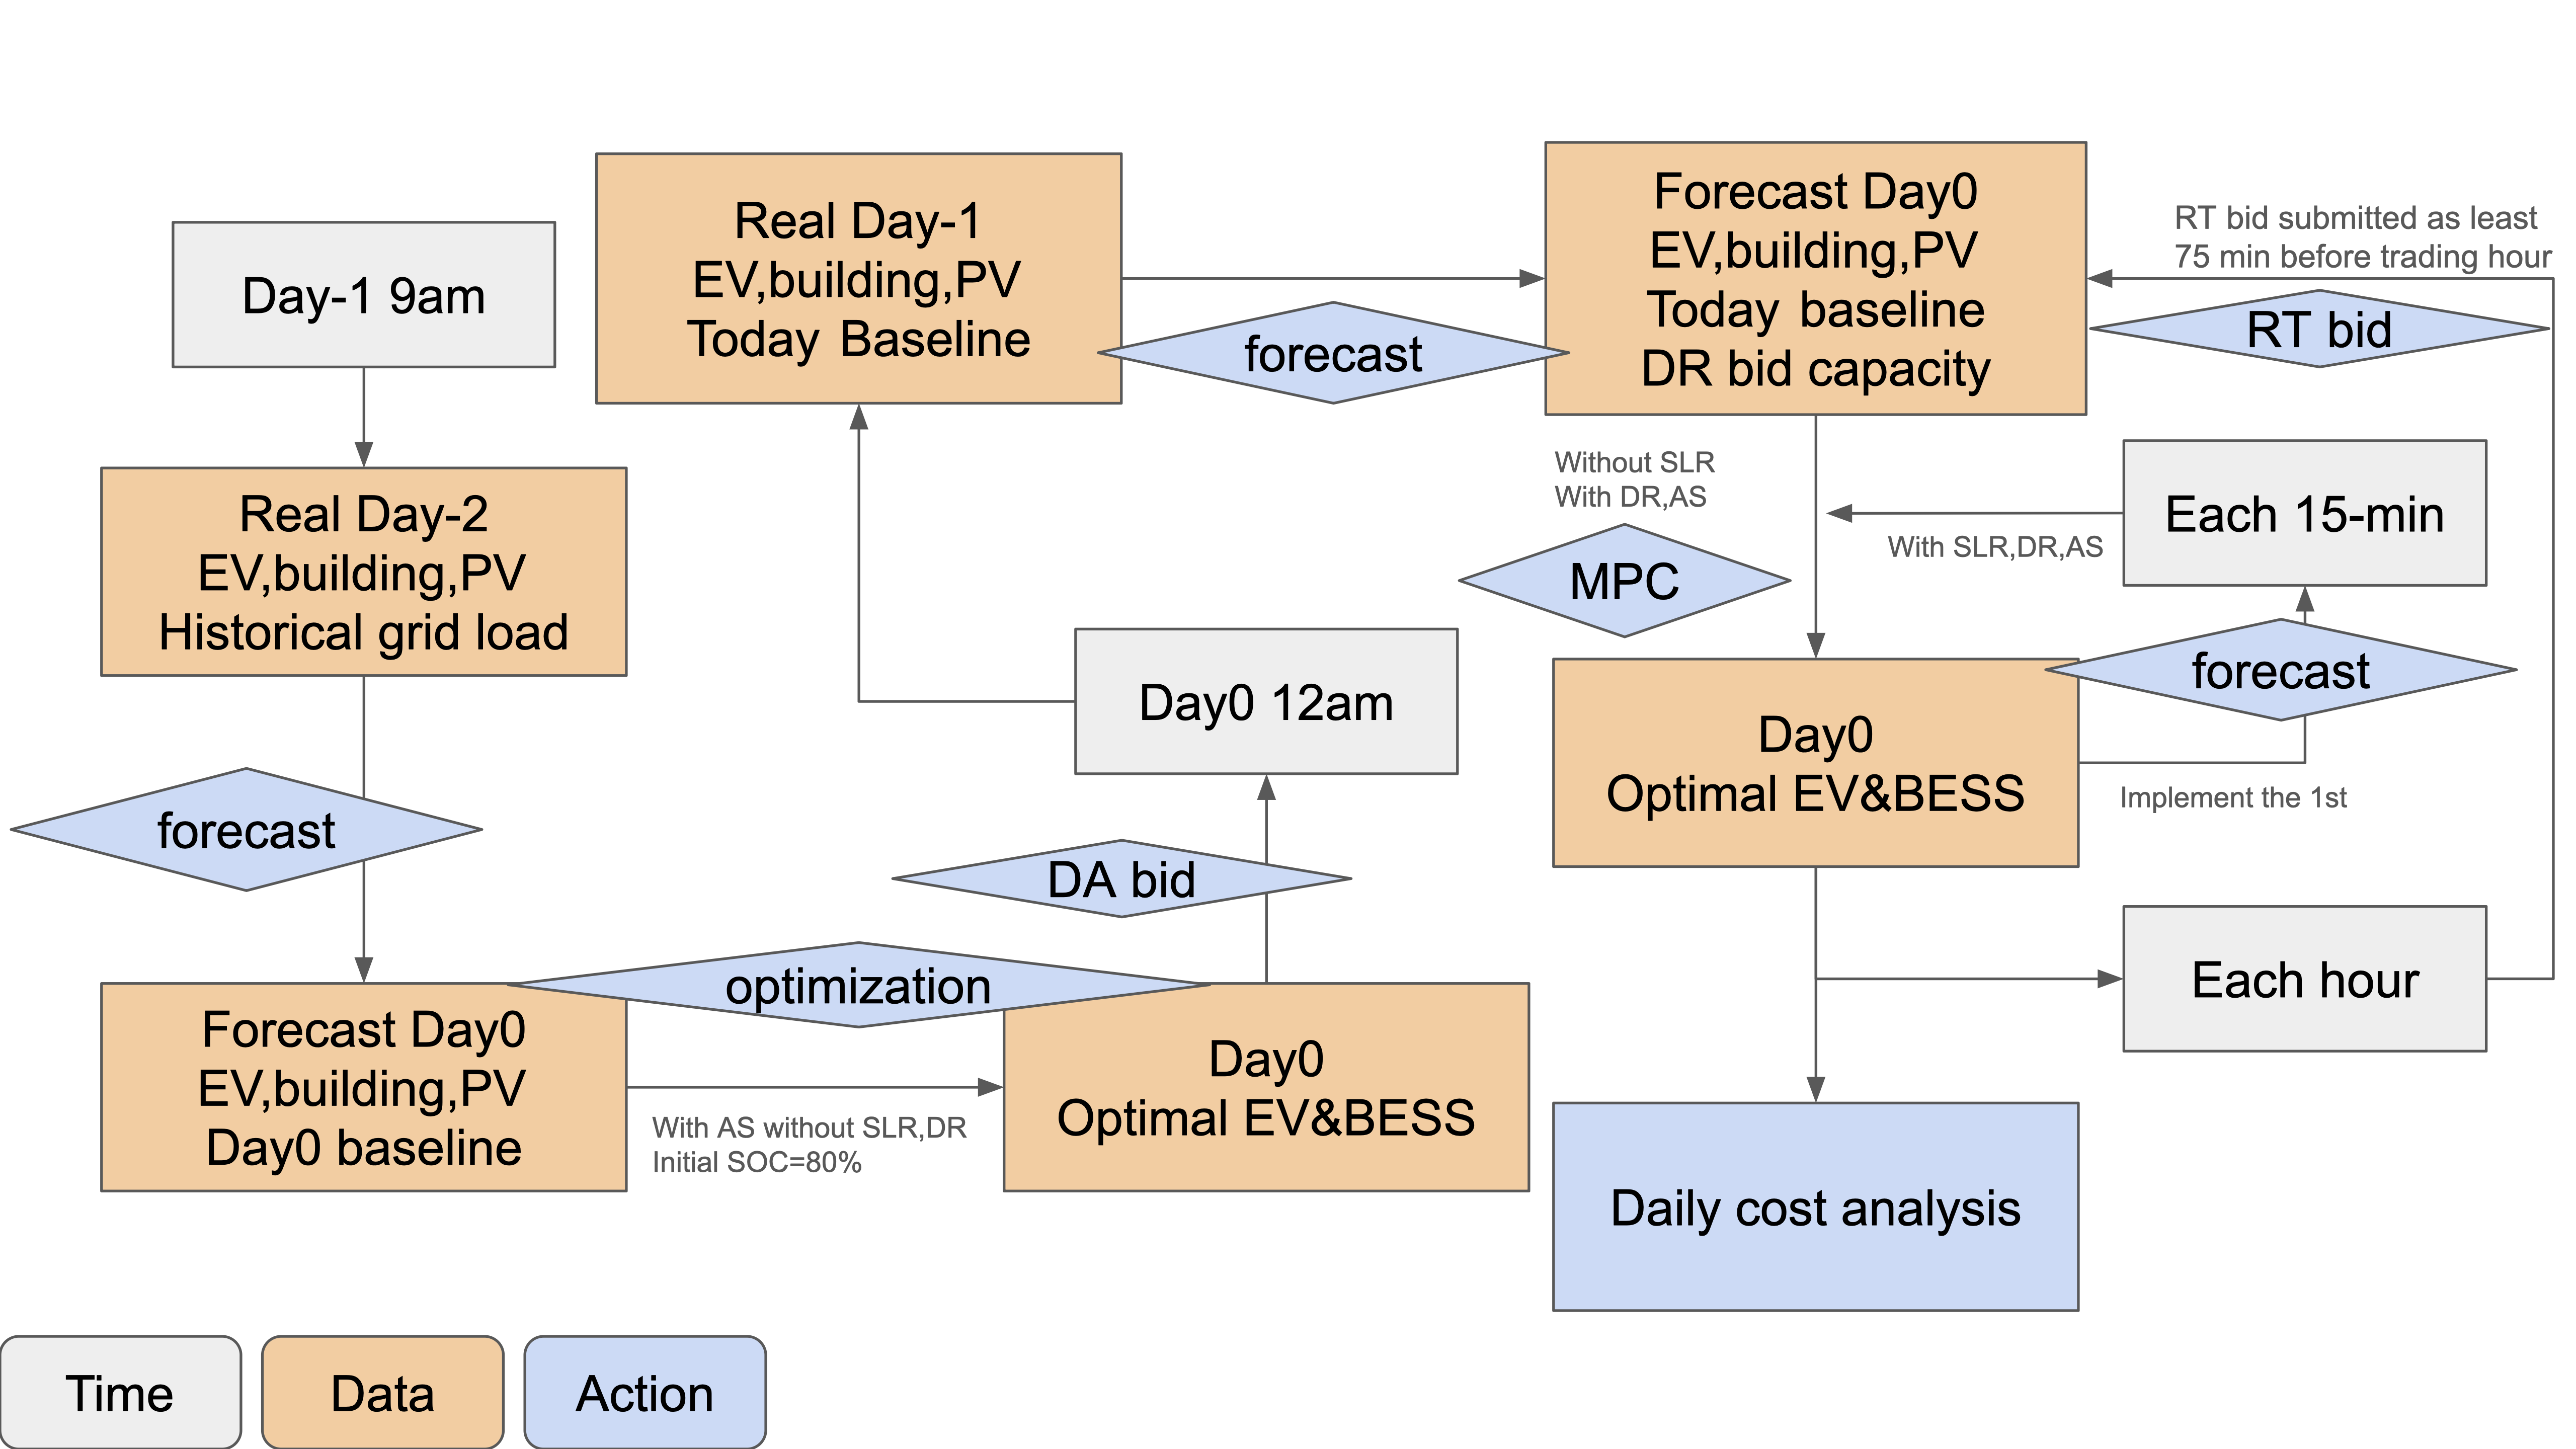
\includegraphics[width=\linewidth]{flowchart.png}
    \caption{Flow chart.}
    \label{fig:flowchart}
\end{figure*}



CAISO requires all customers to submit their DR DA bid before 1000~h on day-1. Therefore, on day-1 at 0900~h we persist the day-2 EV session data to generate a forecast for the day0 EV load, same for the building load and PV. Then we solve an optimization problem with the objective as Eq.~\ref{eq:obj}. The cost contains retail costs of Eq.~\ref{eq:ncd} as non-coincident demand charge, Eq.~\ref{eq:pd} as peak demand charge and Eq.~\ref{eq:tou} as time-of-use charge paid to SDG\&E. All the retail costs are posed on the actual net load of the micro-grid as Eq.~\ref{eq:actual_net_load}, while Eq.~\ref{eq:pd} considers the maximum load in each month, and only happens in daily peak demand hours as Eq.~\ref{eq:z_pd}. One more cost is a virtual penalty of deviation from service level reduction (SLR) of EVs in Eq.~\ref{eq:SLR_penalty}, which encourages moderate reduction of service level to meet the EVs' energy demand and is not an actual payment to either CAISO or SDG\&E. By modifying the $\delta$, we can study the sensitivity to the EV drivers' implicit expectation of the inadequate charging to their vehicles and reach a trade-off between improving the DR revenue and reducing the possible EV charging revenue. On another side, the revenue contains EV driver payment to the aggregator as Eq.~\ref{eq:c_ev}, and the BESS AS capacity revenue as Eq.~\ref{eq:AS_DA_capacity_revenue} which is fixed after bidding. The cost paid by EV drivers to the aggregator in Eq.~\ref{eq:c_ev} is at 0.15$\$/kWh$, and in reality, as of March 30, 2025 $c_{\text{EV}}$ is 0.40$\$/kWh$, but with that large of a rate it would rarely be beneficial to reduce service level and participate in California's energy markets. Therefore, a lower rate is assumed here. 

The optimization problem needs to meet the listed EV and BESS constraints: (a) Eq.~\ref{eq:EV_dynamic} and Eq.~\ref{eq:EV_physical} state the EV dynamic and physical constraints respectively: For each EV the sum of scheduled charging power is the difference of forecast energy demand times SLR, and the power already charged until the current time step. Moreover the charging matrix of the EV fleet is upper-bounded by the maximum energy matrix. Eq.~\ref{eq:z_price}, Eq.~\ref{eq:z_layover} and Eq.~\ref{eq:eta_i} are constraints for SLR decision. These constraints ensure that SLR is only allowed under limited circumstances: (i) the sum of the DA LMP and EV charging rate is higher than the TOU rate, meaning that there is an economic benefit from the reduction in service level; (ii) the target EV for SLR must be present, i.e. the elements in the maximum energy matrix is non-zero; (iii) the current hour is a DR event hour. If all 3 conditions are met, an EV is considered as a candidate of SLR at the current hour. Eq.~\ref{eq:eta_i} proposed a loose constraint in that as long as an EV meets the requirement at 1 out of 24 hours, we can perform SLR to make a profit. (b) Eq.~\ref{eq:BESS_load} introduces a virtual variable as the load of BESS into the micro-grid, Eq.~\ref{eq:bess_dir} ensures two directions of BESS cannot happen at the same time with the binary variable in Eq.~\ref{eq:z_D}, and although in real case BESS can only either charge or discharge, all the capacities can be bid to CAISO. Eq.~\ref{eq:BESS_physical} and Eq.~\ref{eq:BESS_physical2} are state of charge (SOC) physical and dynamic constraints, with a constant number two providing marginal safety and the initial $SOC_t^{\text{BESS}}$ as 80\%. The last BESS constraints are Eq.~\ref{eq:cycle} and Eq.~\ref{eq:cycle_physical} which limit the cycle times and can reduce the degradation cost.



Here are some more details of the optimization: two matrices are introduced and updated at each time step. As shown in Fig.~\ref{fig:EV_matrix} from \cite{chen2024cost}, the maximum energy matrix shows for each EV how much energy could be charged physically during the rest of the day, which is either 0 (EV not on site) or the layover duration times maximum power of the charger (EV on site). The charging matrix $X_{t,\text{opt}}$, also as a decision variable in Eq.~\ref{eq:obj}, has dimensions of $T-t+1 \times N_{\text{EV}}$, and because we already forecast the day0's EV profile, we have the $X_{0,\text{opt}}$ with size $N \times N_{\text{EV}}$ as the output of day0 EV scheduling. During the day0 optimization we also need to forecast building load and PV generation and update the load baseline update for day0, and can hence calculate the optimal net load forecast and capacity for DR by Eq.~\ref{eq:actual_net_load} and Eq.~\ref{eq:DR_capacity} respectively.

\begin{figure}[ht]
    \centering
    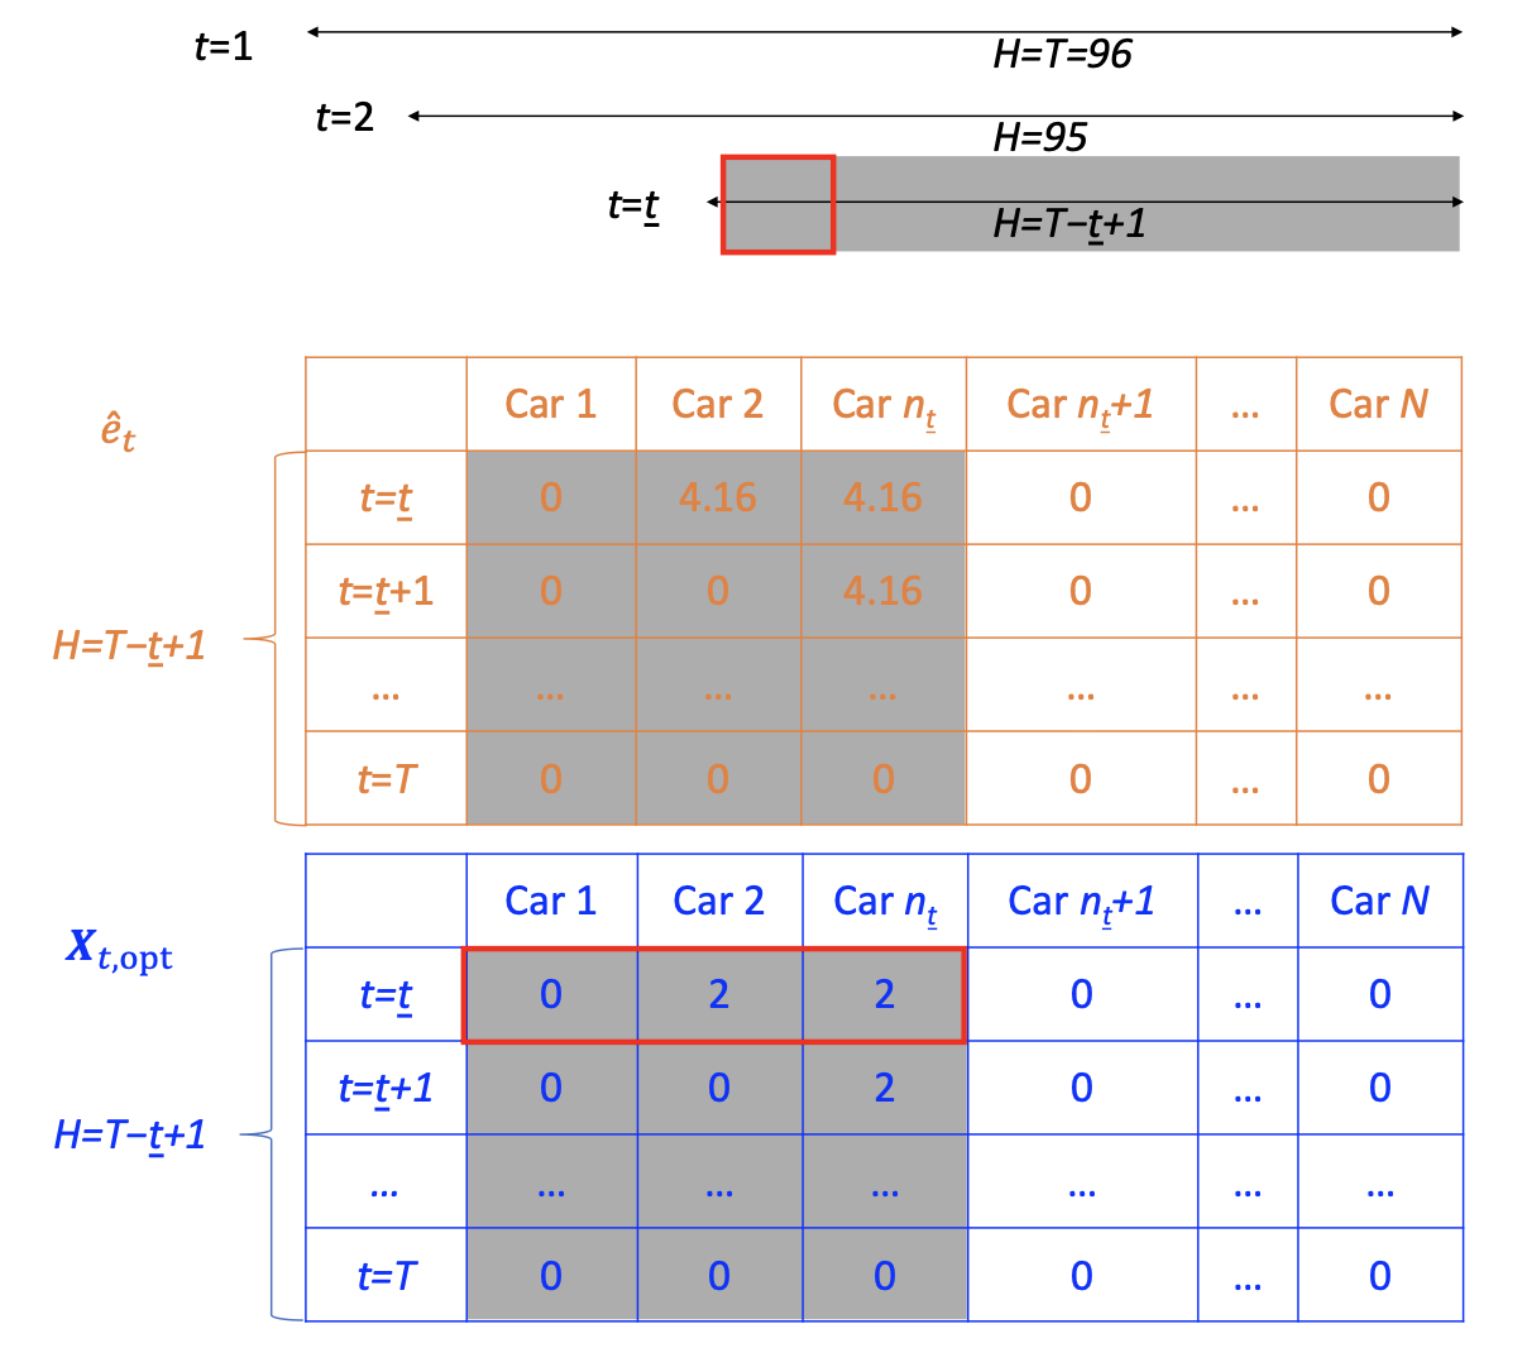
\includegraphics[width=1\linewidth]{EV_charging_matrix.png}
    \caption{EV charging power matrix (bottom) and maximum energy matrix (top).}
    \label{fig:EV_matrix}
\end{figure}

After running the optimization at 0900~h on day-1, we get day0's candidate of optimal EV and BESS scheduling, thus computing day0's hourly bid capacity for the DR market by saving the hourly value of $P_{\text{act},t}^{\text{DR}}$ as $P_{\text{bid}}^{\text{DR}}$ and hence decide the pricing strategy and submit the bidding for day0. The bid capacity can be either positive or negative. DR bids are only submitted if $P_{\text{bid}}^{\text{DR}}$ is positive, i.e. when DR capacity is available. Therefore, we set the bidding price as the floor of that day0 hour's LMP to make sure we win the bid. Otherwise we set it as the legal ceiling price of DRAM as $\bar{c}$. The bidding for AS is similar to DR because they are combined together as a price-capacity bundle to CAISO. The difference is that AS does not have a baseline, so only capacity of each type of AS is bid, which is not a forecast value, but a decision variable by the solver. The AS bid price is set as the floor of DA hourly AS prices. 

\subsection{Real-time Bidding}

Once the bid is accepted by CAISO on day-1 1000~h, the event hour is determined for day0 (today) as Eq.~\ref{eq:DR_event_hour}. At the start of day0 (0000~h) the objective function has more terms: Eq.~\ref{eq:DR_DA_revenue} is the DA DR revenue with DA LMP by RT DR capacity at event hours. Eq.~\ref{eq:DR_settlement} is RT supplemental energy revenue from and RT DR settlement, either revenue or penalty in respect to the real case and baseline. Once CAISO calls upon the DR service, bidders should be penalized if the capacity is lower than bid or be rewarded if they provide excessive capacity, and these adjustments occur in the settlement. Both AS and DR markets include a settlement, and the difference is that the DR performance is evaluated against a baseline, and AS DA bidding has to be strictly met. For DR RT dispatch the difference between actual and bid capacity can be either positive, resulting in a reward for over-performing, or negative, resulting in a penalty for under-performing. However, if the DR energy falls short compared to the bid, which is usually due to an unpredicted increase of demand, which causes the actual load to be closer to or higher than the baseline. If the actual DR energy delivered is still positive, but smaller than what we bid, we pay for the difference. If the actual load is higher than the baseline, CAISO will only charge for not being able to provide the DA bid capacity, but not for the excessive demand increase.

Eq.~\ref{eq:AS_energy_revenue} is the last additional revenue from BESS energy arbitrage and AS mileage performance. In RT realization Eq.~\ref{eq:AS_DA_capacity_revenue} is a fixed value which has to be met, and the RT AS capacity is bid as an excessive part if the DA bidded one is not enough. CAISO will suspend the aggregator if DA bid AS capacities are not met in RT. For the AS deployed energy in Eq.~\ref{eq:AS_energy_revenue}, i.e. mileage performance of frequency regulation up or down and the calling of operating reserve, is controlled by the AGC signal sent by CAISO each 4 seconds. It would take too much computing resources to follow the same resolution in the optimization to compute the energy payment by each signal. Therefore, we assume that the regulation efficiency (the amount in which the reserved capacity is deployed) and the operating indicator (whether spinning or non-spinning reserve is called at the current time step) are known. By introducing the regulation efficiencies, we approximate the real payment of the 4-s AGC signal in the 15-min problem. 



At the start of each 15 minutes of day0, namely 0000~h, 0015~h, etc. until 2345~h. At each time step we keep the objective function and constraints in the problem the same, but run the optimization again to get more updated optimal results of future EV schedule and BESS dispatch. With the recursive updates, we can then submit RT bids at the end of each 15 minutes. The bidding process remains the same as DA but follows a different time schedule: at 2200~h day-1 we make the first RT bidding which influences the time period from 0000~h to 0100~h day0 etc, because RT bids have to be submitted at least 75 minutes (we choose 2 hours) before the operating hour. At each time step we forecast, optimize, implement the next time step's optimal schedule and bid, which forms an update framework.

Only Eq.~\ref{eq:DR_settlement} is impacted with the bid variables as--aside from the RT settlement--all other objective function terms only include RT capacities and loads. Therefore the introduction of RT bidding does not significantly change the final cost and decision-making of the solver, but is a remedy for inaccurate forecast, which can happen if we apply persistence forecast for all variables but there are large day-to-day changes.





\subsection{Algorithm}
\vspace{0.5em}
\noindent
\textbf{Optimization Processes:}
\begin{enumerate}
    \item \textbf{Day-1 at 09:00 (Execution Time)} – preparing for Day0 operations:
    \begin{itemize}
        \item Load Day-2 data: EV dispatch, building load, and PV generation data \hfill (Data used for forecasting Day0)
        \item Initialize BESS with 80\% SOC \hfill (Applies immediately)
        \item Forecast Day0 EV load, building load, and PV generation \hfill (Forecast valid for Day0 00:00–24:00)
        \item Solve optimization without DR to get baseline, EV load and BESS dispatch \hfill (Plan valid for Day0)
        \item Submit Day0 capacity bid to Day-1's market before 10:00 \hfill (Bid applies to Day0)
    \end{itemize}

    \item \textbf{Day-1 at 22:00, 23:00 (Execution Time)} – preparing for Day0 operations:
    \begin{itemize}
        \item Submit RT AS bids (Bid applies to Day0)
    \end{itemize}
    
    \item \textbf{Day0 (Execution Time)} – real-time operation and market participation:
    \begin{itemize}
        \item \textbf{00:00 (Execution Time)}
        \begin{itemize}
            \item Load Day-1 final BESS SOC, DR event hours, actual EV dispatch, grid baseline, building load, and PV generation (Applies to Day0 at 00:00)
            \item Forecast Day0 load again, building load, and PV generation (Valid for Day0 00:00–24:00)
            \item Solve optimization with DR and AS market participation enabled (Plan applies to 00:00–24:00)
            \item Submit RT market bid for 02:00–03:00 (Valid for next hour)
            \item Implement MPC output (EV load dispatch, BESS operation) for 00:00–00:15 (Applies at 00:00 immediately)
        \end{itemize}
        
        \item \textbf{00:15–23:45 (Repeated Every 15 min)}:
        \begin{itemize}
            \item Update forecasts with real-time measurements (e.g., SOC, EV sessions, PV) (Applies from current time step to 24:00)
            \item Run rolling MPC with updated market with SLR (Plan applies to 24:00)
            \item Submit RT market bid for 2 hours later interval (e.g., 02:15–02:30 at 00:15)
            \item Implement MPC outputs for current 15-min interval (Applies immediately)
        \end{itemize}

         \item \textbf{09:00 (Execution Time)}:
        \begin{itemize}
            \item Prepare Day+1 DA bidding as before \hfill (Plan valid for Day+1)
        \end{itemize}
    \end{itemize}
    
    \item \textbf{Day0 Settlement (Execution Time: 23:45)}:
    \begin{itemize}
        \item Analyze revenues and costs from DR and AS \hfill (Covers Day0 results)
        \item Archive results and prepare for next day’s DA bidding (Affects Day+1 planning)
    \end{itemize}
\end{enumerate}




\section*{Acknowledgment}
This research is funded by TotalEnergies as part of a collaborative project with the University of California, San Diego.



\printbibliography


\end{document}
